\subsection{实验目的-搭建 iptables 实验环境}
搭建 iptables 实验环境.
%
\subsection{实验原理}
VMware Workstation 软件包含一个用于英特尔 x86 兼容计算机的虚拟机套装,
其允许多个 x86 虚拟机同时被创建和运行。每个虚拟机实例可以运行其自己的客
户机操作系统。VMware 工作站允许一台真实的计算机同时运行数个操作系统。
%
\subsection{实验环境}
软件:
\begin{itemize}
  \item VMware
  \item 操作系统:
    \begin{itemize}
      \item Windows 7
      \item Windows server 2003
      \item CentOS 6.5
      \item CentOS 6.5
    \end{itemize}
\end{itemize}
%
设备拓扑图:
\begin{figure}[H]
  \begin{center}
    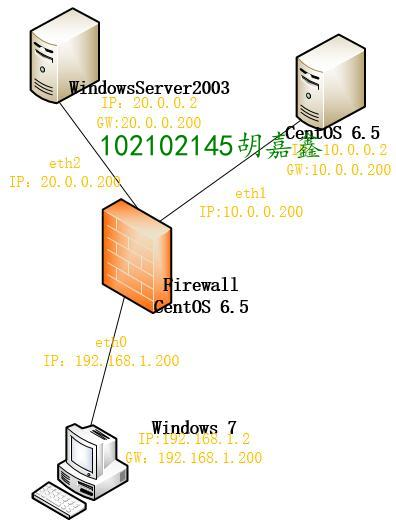
\includegraphics[width=0.40\textwidth]{2_1_1.jpeg}
  \end{center}
\end{figure}
%
\subsection{实验步骤}
\subsubsection{配置虚拟机 IP 地址}
将操作机 Windows 7 的 IP 地址设置为 \texttt{192.168.1.2},
子网掩码设为 \texttt{255.255.255.0},
默认网关设为 \texttt{192.168.1.200}。
\begin{figure}[H]
  \begin{center}
    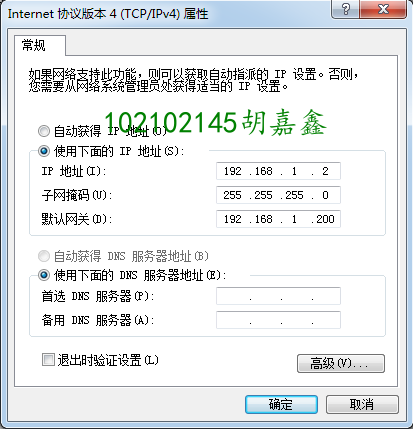
\includegraphics[width=0.40\textwidth]{2_1_2.png}
  \end{center}
\end{figure}

将 Windows server 2003 的 IP 地址设为 \texttt{20.0.0.2},
子网掩码设为 \texttt{255.255.255.0},
默认网关设为 \texttt{20.0.0.200}。
\begin{figure}[H]
  \begin{center}
    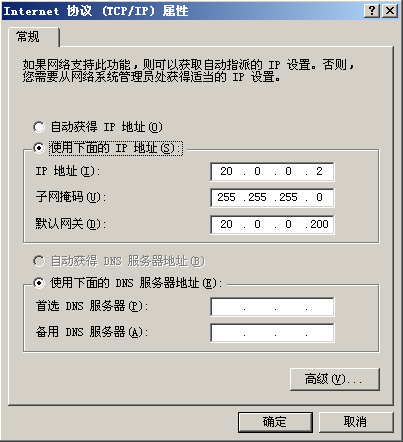
\includegraphics[width=0.40\textwidth]{2_1_3.png}
  \end{center}
\end{figure}

将服务器 CentOS 6.5 的 IP 地址设置为 \texttt{10.0.0.2},
子网掩码设为 \texttt{255.255.255.0},
网关设为 \texttt{10.0.0.200}。
\begin{figure}[H]
  \begin{center}
    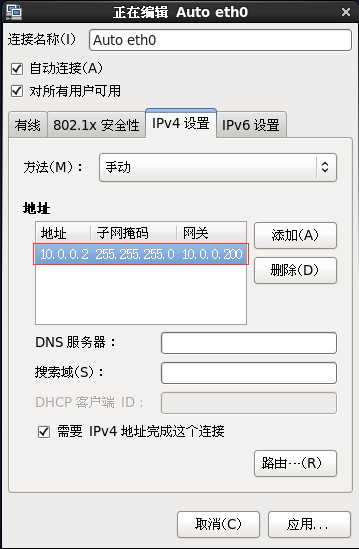
\includegraphics[width=0.40\textwidth]{2_1_4.png}
  \end{center}
\end{figure}

作为防火墙的另一台 CentOS 6.5 安装了 3 块网卡,将网卡 eth0 的 IP 地址
设置为 \texttt{192.168.1.200},
将网卡 eth1 的 IP 地址设置为 \texttt{10.0.0.200},将网卡 eth2
的 IP 地址设置为 \texttt{20.0.0.200},
3 块网卡的子网掩码都设置为 \texttt{255.255.255.0}。
\begin{figure}[H]
  \begin{center}
    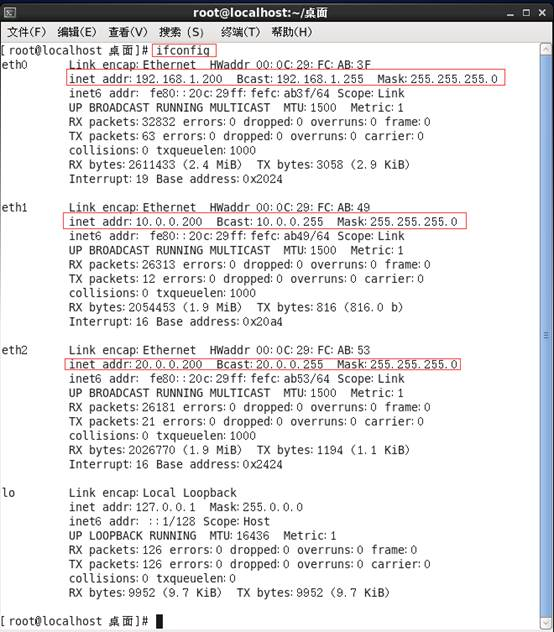
\includegraphics[width=0.40\textwidth]{2_1_5.jpeg}
  \end{center}
\end{figure}

开启网卡之间的 IP 转发功能,在终端输入命令
\begin{minted}[bgcolor=bg]{sh}
echo "1" > /proc/sys/net/ipv4/ip_forward
\end{minted}
再输入命令
\begin{minted}[bgcolor=bg]{sh}
cat /proc/sys/net/ipv4/ip_forward
\end{minted}
可以看到 \mintinline[breaklines=true]{sh}{/proc/sys/net/ipv4/ip_forward} 中数值为 1,
说明 IP 转发功能已经打开。
\begin{figure}[H]
  \begin{center}
    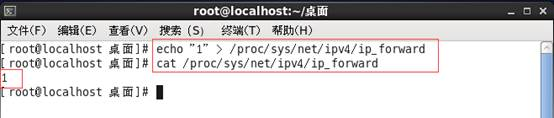
\includegraphics[width=0.40\textwidth]{2_1_6.jpeg}
  \end{center}
\end{figure}

要想永久使用 IP 转发,需要修改 \mintinline[breaklines=true,breakbytoken=true]{sh}{/etc/sysctl.conf} 文件,
修改下面一行的值:
\begin{minted}[bgcolor=bg]{sh}
net.ipv4.ip_forward=0
\end{minted}
将 0 改为 1。修改后可以重启系统来使修改生效,
也可以执行命令
\begin{minted}[bgcolor=bg]{sh}
sysctl -p /etc/sysctl.conf
\end{minted}
来使修改生效。
%
\subsubsection{测试 win7、2003 和服务器 centos 的是否连通}
在操作机 Windows 7 上打开 cmd,
分别输入命令``\texttt{ping 10.0.0.2}''和
``\texttt{ping 20.0.0.2}'',都可以 ping 通。
\begin{figure}[H]
  \begin{center}
    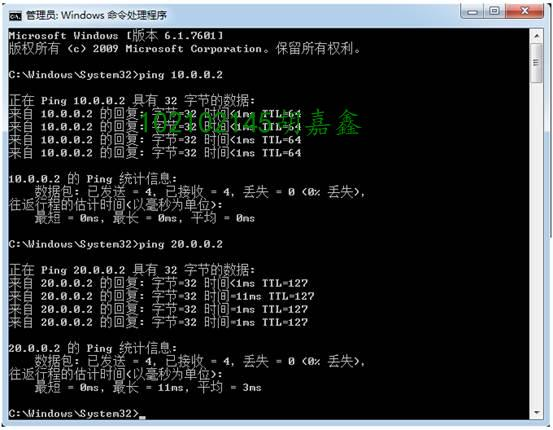
\includegraphics[width=0.40\textwidth]{2_1_7.jpeg}
  \end{center}
\end{figure}

在 Windows server 2003 上打开 cmd,分别输入命令
``\texttt{ping 192.168.1.2}''
和``\texttt{ping 10.0.0.2}'',都可以 ping 通。
\begin{figure}[H]
  \begin{center}
    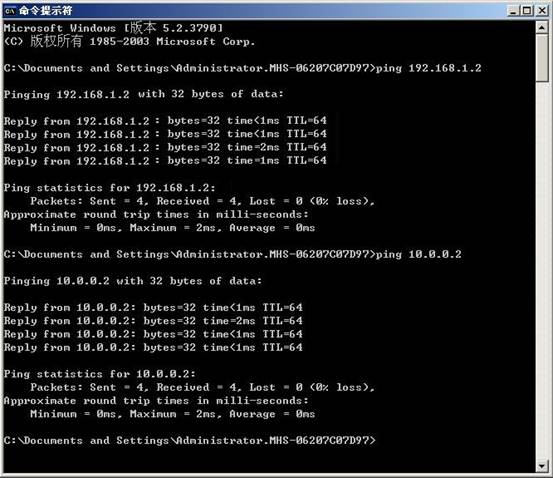
\includegraphics[width=0.40\textwidth]{2_1_8.jpeg}
  \end{center}
\end{figure}

在服务器 CentOS 6.5 上打开终端,
分别输入命令``\texttt{ping 192.168.1.2}''和
``\texttt{ping 20.0.0.2}'',都可以 ping 通。
\begin{figure}[H]
  \begin{center}
    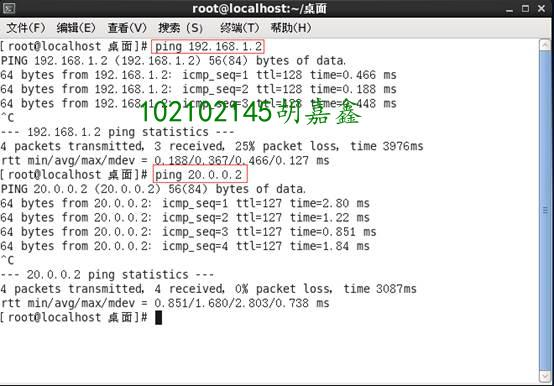
\includegraphics[width=0.40\textwidth]{2_1_9.jpeg}
  \end{center}
\end{figure}

至此,成功搭建完 iptables 的实验环境。
%
